\chapter{Desarrollo}
\label{chapter:Desarrollo}

En esta parte de la memoria se detallarán los pasos seguidos durante el desarrollo y la aplicación de los algoritmos de \textit{Machine Learning} sobre los datos utilizados. Asimismo, se profundizará en los datos utilizados y cómo se han preprocesado para su posterior aplicación en los algoritmos.

Generalmente, la mayor parte del tiempo de un proyecto de \textit{Data Science} se invierte en la extracción y preprocesado de los datos, hasta que tengan la suficiente calidad como para arrojar resultados fiables tras aplicar los algoritmos. Este ha sido el caso del presente proyecto, la mayor parte de los esfuerzos han recaído en la comprensión de los datos y en cómo hacer frente (tanto por tiempo como por tamaño) a los datos disponibles.

Tanto el preprocesado como la aplicación de los algoritmos de \textit{Machine Learning} se han realizado utilizando el lenguaje de programación \textit{Python} en su versión 3.6 y la exploración y análisis de los datos se han realizado en \textit{Jupyter Notebooks} para facilitar la visualización de los datos y las acciones tomadas. Todo estos procesos se han realizado en una máquina remota proporcionada por la UOC con 10 núcleos y 64gb de memoria RAM.
\newpage

\section{Datos utilizados}

Para este proyecto se va a utilizar un \textit{dataset} con información de las conexiones entre dispositivos IoT, mediante el análisis de los paquetes obtenidos por un analizador de paquetes o \textit{sniffer}, un software que permite observar y recopilar las acciones que desarrollan dentro de una red \cite{sniffer}. Utilizando los datos recopilados por este software se preprocesarán de modo que se pueda extraer la información y posteriormente transformarla y crear nuevas variables.

Los datos iniciales fueron preprocesados inicialmente con la información de las anomalías (únicamente anomalías) que se habían recopilado en un espacio de tiempo de dos meses. En este caso los datos solo contaban con tráfico ilegítimo, por lo que no se podía hacer una detección de anomalías como tal.

Posteriormente, se proporcionaron los datos en bruto en un fichero de extensión \textit{pcap} resultante del \textit{sniffer} mencionado anteriormente. Este fichero contiene información de las distintas capas en las que se almacenan los datos, siendo las de más interés las capas \textit{TCP} e \textit{IP}.

\begin{itemize}
    \item \textit{Transmission Control Protocol}: originario de los años 70/80, consiste en un protocolo para la transmisión de paquetes en conexiones \textit{host} a \textit{host} en redes \cite{postel1981transmission}.
    \item \textit{Internet Protocol}: protocolo que permite la transmisión de datos de origen a destino donde el origen y el destino son direcciones de longitud fija y proporciona los medios para la división y reagrupación de grandes datos en grupos más pequeños \cite{postel1981internet} .
\end{itemize}

Sobre estas capas se obtiene la información disponible al más bajo nivel y posteriormente se generarán nuevas variables en base a los datos obtenidos. Siendo los datos de la capa TCP los siguientes:

\begin{itemize}
    \item Puerto de origen: indica el puerto de origen utilizado para realizar la conexión desde la IP de origen.
    \item Puerto de destino: indica el puerto de destino utilizado en la conexión entre \textit{hosts}.
\end{itemize}
\newpage

Los datos obtenidos de la capa IP:
\begin{itemize}
    \item IP de origen: dirección con longitud fija del origen de la conexión.
    \item IP de destino: dirección con longitud fija del destino de la conexión.
    \item \textit{Length}: longitud/tamaño de los paquetes enviados durante la conexión.
\end{itemize}

\begin{figure}[H]
    \centering
    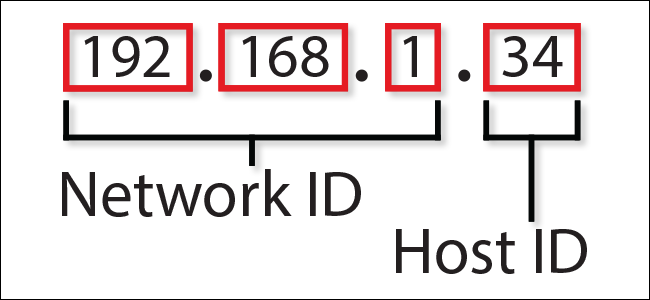
\includegraphics[width=6cm]{figs/ip.png}
    \caption{Ejemplo de dirección IPv4}
    \label{fig:wireshark}
\end{figure}

Otros datos:

\begin{itemize}
    \item \textit{Payload}: contenido de los datos transmitidos, pudiendo ser texto, imágenes o comandos a ejecutar en el \textit{host} de destino, con posibilidad de estar cifrado.
    \item \textit{Timestamp}: marca de tiempo que indica en qué momento se realizó la conexión.
\end{itemize}

Un ejemplo más visual de los datos a bajo nivel se puede realizar utilizando la herramienta \textit{Open Source, Wireshark}, fundamental a la hora de entender cómo están distribuidos los datos en las capas.

\begin{figure}[H]
    \centering
    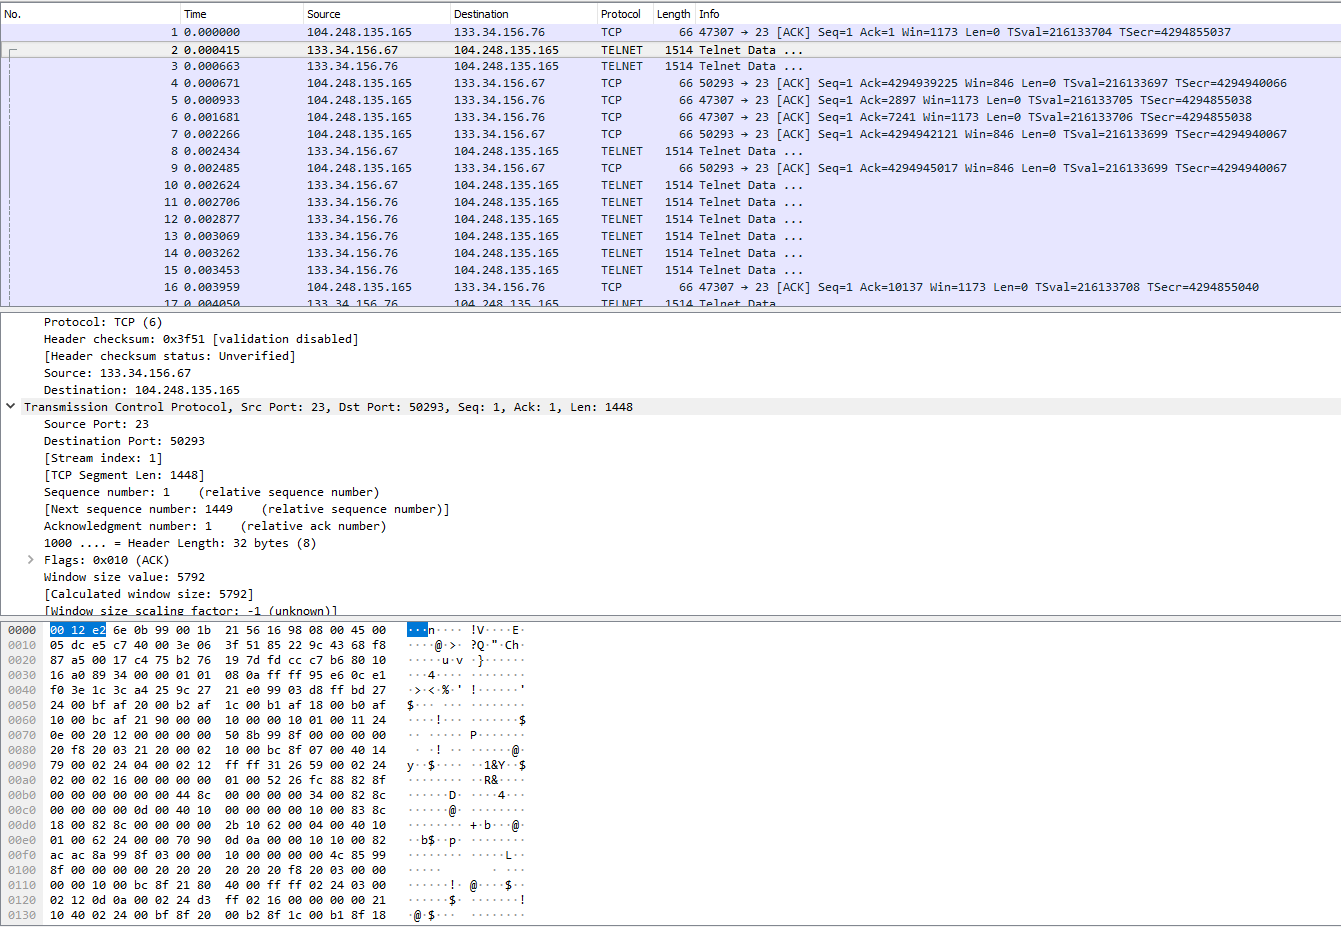
\includegraphics[width=15cm]{figs/wireshark.PNG}
    \caption{Ejemplo de datos pcap en Wireshark}
    \label{fig:wireshark}
\end{figure}

El \textit{Timestamp} puede indicar que el problema debería tratarse como una serie temporal y generar variables en base a esta característica.

Los datos provienen de la recolección de información realizada el 2 de Febrero de 2019, contando tanto con tráfico legítimo como ilegítimo. Sin embargo, no existe clasificación de los datos, por lo que se trata de un problema de carácter no supervisado y como consecuencia se utilizarán técnicas como las descritas en el capítulo \ref{chapter:Estado del Arte} de aprendizaje no supervisado.

\newpage

\section{Exploración y Preprocesamiento}

En este aportado se van a mostrar los pasos seguidos durante la exploración y  el procesamiento asicomo la información obtenida durante el proceso. Ambas etapas se realizan de manera conjunta, es decir, la exploración conlleva la realización de distintos preprocesamientos o otras palabras, se realiza \textit{Feature Engineering}. Se puede definir como el proceso de exploración y procesamiento de datos que ayudan a la creación de nuevas variables que puedan mejorar la eficiencia del modelo\cite{fe}.

El paso inicial era la extracción de los datos del fichero \textit{pcap}, el tamaño total era cercano a los 14 GB, de modo que en el momento de cargar la información en memoria, el uso aumentaba considerablemente dificultando su manipulación, por lo que el primer paso fue investigar si existía alguna forma de dividirlo. El resultado fue el uso de la herramienta \textit{tcpdump}, una línea de comandos utilizada para el análisis de paquetes escrita en C/C++ \cite{tcpdump}, la misma permitía la división del fichero original en pequeños ficheros con el tamaño deseado. La división se realizó con un tamaño máximo de 500 MB, para permitir la posterior paralelización de los ficheros y evitar un uso muy alto de memoria, dando como resultado 15 ficheros.

Una vez obtenidos los ficheros se deben procesar de modo que el resultado sean datos de forma tabular, que puedan ser explorados y preprocesados con mayor facilidad. Para realizar este proceso se utilizó el módulo de \textit{python}, \textit{scapy}, utilizado comúnmente en tareas de análisis de redes. Gracias a la granularidad de los nuevos ficheros y a utilizar \textit{python} se procesan 9 ficheros simultáneamente utilizando el módulo mencionado, éste se encarga de recorrer las capas mencionadas y extraer los datos y organizarlos de forma tabular, concretamente en \textit{csv}. En ciertos casos, los paquetes pueden contener el \textit{payload}, cuando este es el caso se extrae y se añade como una columna más, para el resto se trata como si fueran \textit{NA} o datos sin registro. 

Una vez terminado el proceso se obtienen los primeros datos en brutos de carácter estructurado. Se genera una cantidad análoga de ficheros con un volumen tres veces superior a los datos originales, con las variables mencionadas en la sección anterior. Antes de realizar ningún tipo de exploración se realiza un preprocesado en paralelo para generar nuevas variables sencillas que puedan aportar información de cara a la primera exploración. Las nuevas variables son las siguientes:

\begin{itemize}
    \item Red 1 IP origen
    \item Red 2 IP origen
    \item Red 3 IP origen
    \item Host IP origen
    \item Red 1 IP destino
    \item Red 2 IP destino
    \item Red 3 IP destino
    \item Host IP destino
    \item is\_busybox
    \item is\_sh
    \item is\_enable
\end{itemize}

Las variables en referencia a las IPs se generaron haciendo una división de las direcciones:

\begin{equation}
    192.168.1.1 => 192_{red1}\; 168_{red2}\; 1_{red3}\; 1_{host}
\end{equation}

El resto de las variables se obtuvieron mediante el \textit{parseo} del \textit{payload} en aquellos registros que así lo tuvieran y buscando la existencia de las palabras clave \textit{sh, enable y busybox}, siendo la mayor parte de los registros sin contenido en el \textit{payload} o incluso cifrado. La razón por la que se eligieron estas palabras clave es por el uso de este tipo de comandos en los dispositivos IoT por \textit{malwares} conocidos, \textit{busybox} se trata de una versión mínima de un sistema operativo \textit{UNIX} utilizado en pequeños dispositivos y que puede ser explotado por \textit{malware}\cite{ibmiot}.  De la misma manera \textit{sh} y \textit{enable} son comandos comúnmente utilizados en este tipo de ataques. Las tres variables son de tipo binario, es decir, indica si en el registro existe el comando o no.

El proceso de exploración se realiza en \textit{Jupyter Notebooks} con la ayuda del módulo \textit{matplotlib} y \textit{seaborn} para las visualizaciones. Para esta primera exploración, se van a buscar los medios más utilizados en las distintas conexiones, es decir, las IPs más utilizadas, puertos más utilizados, información de las variables binarias y la evolución de la cantidad de conexiones en el tiempo.

\begin{figure}[H]
    \centering
    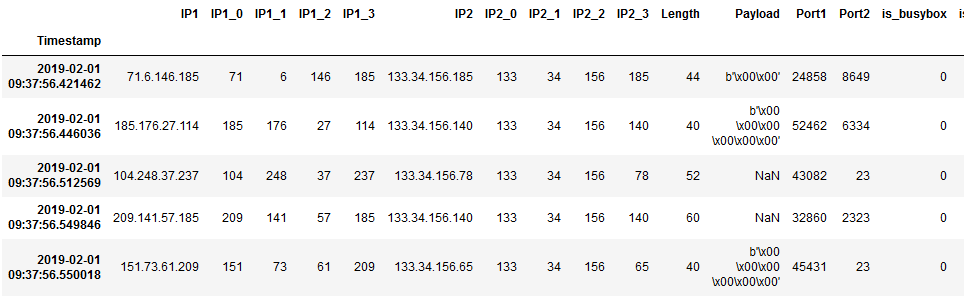
\includegraphics[width=15cm]{figs/initial_data.PNG}
    \caption{Datos en forma tabular}
    \label{fig:tabulardata}
\end{figure}

Para realizar la exploración se unen todos los datos contenidos en los ficheros generados ordenados por la marca de tiempo. Una vez cargados, se realizan las operaciones básicas para determinar que no faltan datos, es decir, que en las variables originales (salvo el \textit{payload}) no falta ningún tipo de registro. En este caso no hay existencia de \textit{NAs} en las variables, en otras palabras, todos los datos tienen los registros necesarios.

En la siguiente gráfica se puede observar la cantidad de valores únicos en cada variable, en la que se pueden apreciar dos cosas claras:

\begin{itemize}
    \item Las variables con más únicos son las de los puertos.
    \item No hay una gran cantidad de IPs únicas.
\end{itemize}

\begin{figure}[H]
    \centering
    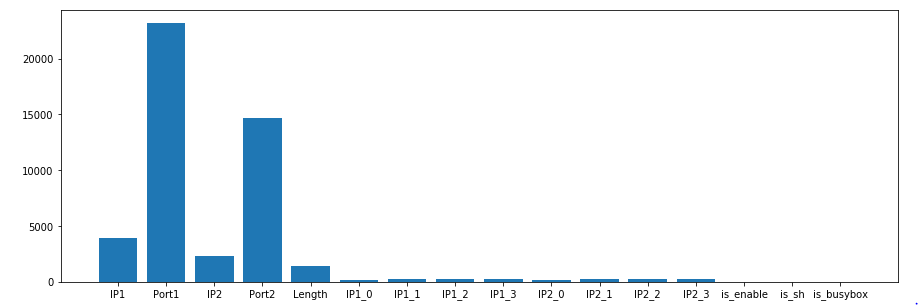
\includegraphics[width=17cm]{figs/unique_vals.PNG}
    \caption{Cantidad de valores únicos en las variables}
    \label{fig:uniquevals}
\end{figure}

La parte de los puertos en origen (subíndice 1) tiene sentido que sea mayor que en la IP destino, dado que a la hora de iniciar conexiones por lo general el puerto origen es aleatorio y el de destino suele ser fijo, como el puerto 22 para conexiones \textit{ssh}, por lo que puede significar que se estuviera haciendo un escaneo de puertos. Esto se puede ver en el diagrama de barras representando los puertos más utilizados en origen y destino:


\begin{figure}[H]
    \centering
    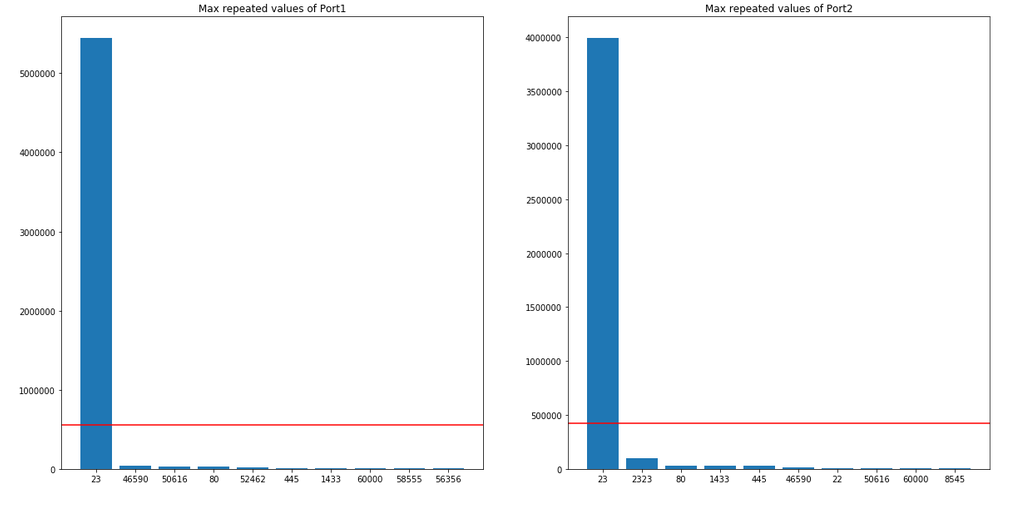
\includegraphics[width=17cm]{figs/ports.PNG}
    \caption{Puertos más utilizados}
    \label{fig:ports}
\end{figure}

Se puede observar lo siguiente:

\begin{itemize}
    \item EL puerto más utilizado en ambos casos con diferencia es el puerto 23. Es el puerto utilizado para realizar las conexiones vía \textit{telnet}.
    \item Seis de los diez puertos más utilizados en la IP de origen son puertos aleatorios, utilizados al realizar la conexión. Los puertos del rango 4xxxx-6xxxx caen en este uso efímero.
    \item El puerto 80 por lo general es utilizado en conexiones \textit{HTTP} (web).
    \item El puerto 445 es utilizado para la transferencia de ficheros.
    \item El puerto 1433 suele utilizarse en conexiones de \textit{Microsoft SQL Server}.
    \item El 2323 puede ser un puerto alternativo para la conexión vía \textit{telnet}\cite{telnetport}.
    \item El puerto 22 se utiliza para conexiones \textit{ssh}.
    \item Tanto para destino como para origen se repiten los puertos 46590, 50616 y 60000, cayendo en el rango de puertos temporales.
\end{itemize}

En el caso de las IPs más utilizadas se puede ver lo siguiente:

\begin{figure}[H]
   \begin{minipage}{0.48\textwidth}
     \centering
     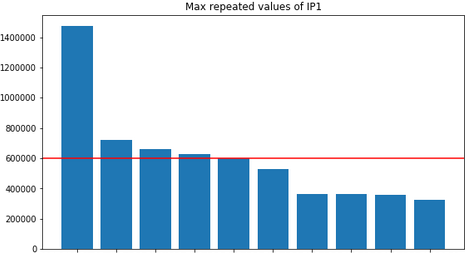
\includegraphics[width=1\linewidth]{figs/ip1.PNG}
     \caption{IPs de origen con la mayor cantidad de conexiones}
     \label{Fig:ip1}
   \end{minipage}\hfill
   \begin{minipage}{0.48\textwidth}
     \centering
     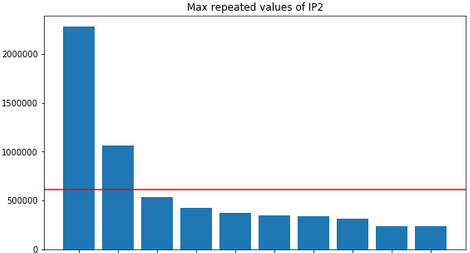
\includegraphics[width=1\linewidth]{figs/ip2}
     \caption{IPs de destino con la mayor cantidad de conexiones}
     \label{Fig:ip2}
   \end{minipage}
\end{figure}

Con una cantidad de datos cercana a los 11 millones de registros la mayor parte de las conexiones se registran en estos diez valores máximos con una diferencia de casi el doble de la primera a la segunda tanto para origen como destino.

Dentro de la temporalidad de las conexiones se pueden observar patrones de las conexiones a lo largo del día y su evolución. Debido a la granularidad de los tiempos (capturan con un detalle de microsegundos) estos patrones se han agrupado en distintas ventanas, de modo que en ventanas más pequeñas se puedan detectar ascensos y descensos bruscos, mientras que en las ventanas grandes se puede observar el patrón general. Por ello se han realizado gráficas con ventanas de 1 minuto, 5 minutos y 30 minutos.

\begin{figure}[H]
    \centering
    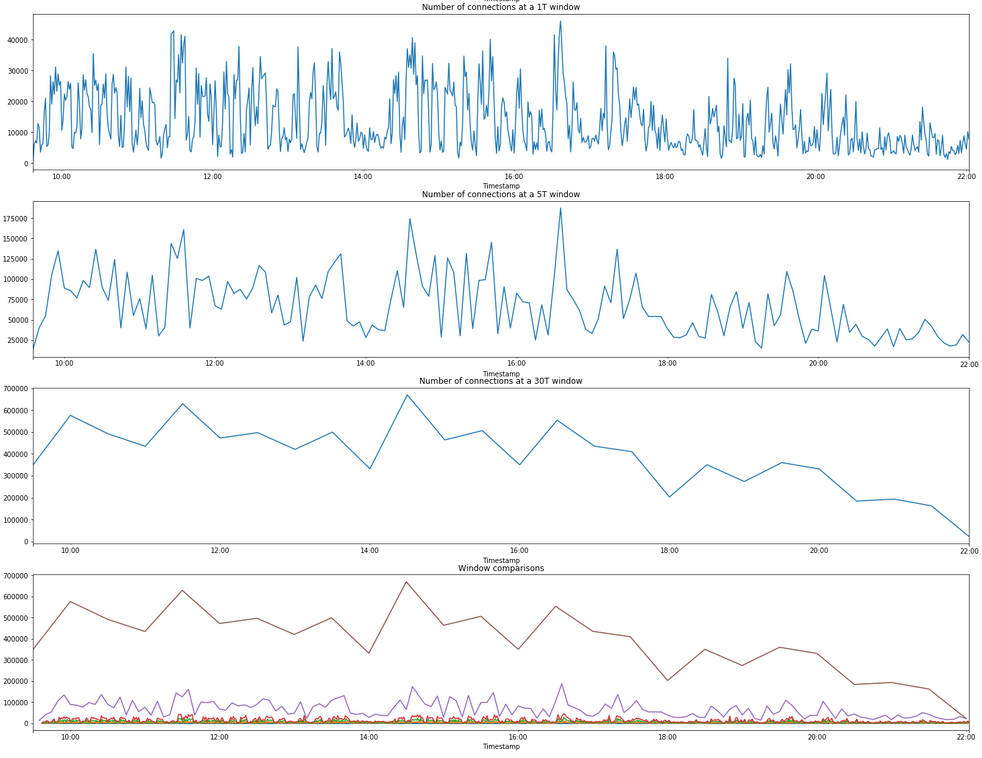
\includegraphics[width=17.5cm]{figs/daily_connections.PNG}
    \caption{Evolución de las conexiones a lo largo del tiempo con distintas ventanas}
    \label{fig:dailyconn}
\end{figure}

Se observa:

\begin{itemize}
    \item Un patrón claro de la cantidad de conexiones, comienza a aumentar durante la mañana y la cantidad de peticiones disminuye por la tarde, lo que puede indicar que la carga en los dispositivos se realiza
\end{itemize}